\documentclass[journal,10pt]{IEEEtran}
\usepackage{amsmath,amssymb,graphicx,booktabs,cite,url,balance}
\newcommand{\BR}{balanced+rare}
\title{Rare-Attack-Aware Balanced Replay for Federated Continual Intrusion Detection in EV Charging Networks}
\author{Author names and affiliations to be confirmed%
\thanks{Working draft, 27 October 2026. Author list, affiliations, contact details, and final submission declarations remain to be completed.}}
\markboth{Working Draft---27 October 2026}{Replay Allocation for Continual Intrusion Detection}
\begin{document}
\maketitle
\begin{abstract}
Small replay memories must preserve earlier intrusion patterns while retaining infrequent attacks. We combine a fixed rare-group reservation with class-balanced local replay for continual flow classification in electric-vehicle charging networks. On the original split, at 60 examples per client, the policy improves old-attack accuracy by 1.53 percentage points and Slowloris recall by 5.06 points over class-balanced replay. Both gains remain significant under federation on each additional split. The study uses merged-Scan primary scores and exact-type sensitivity on one charging dataset with constructed client profiles.
\end{abstract}
\begin{IEEEkeywords}
Federated learning, continual learning, intrusion detection, replay memory, electric vehicle charging.
\end{IEEEkeywords}

\section{Introduction}
Charging stations rely on networked control and monitoring, making sustained communication availability a security concern~\cite{ocpp,dataset}. Low-rate denial-of-service behavior such as Slowloris motivates retaining attack knowledge even when its traffic appears infrequently at individual stations. Our experiments concern recognizing labeled Slowloris flows as new attack cohorts arrive; the operational consequence motivating detection is disruption of charging-related services.

Federated learning supports a shared detector trained from locally retained traffic. D\"IoT demonstrates federated IoT anomaly detection~\cite{diot}, while Kitsune studies online traffic anomaly detection~\cite{kitsune}. Continual intrusion detection additionally needs to preserve earlier labeled attacks; augmented memory replay explicitly addresses imbalance in IDS~\cite{amr}. These lines motivate studying allocation of small local replay memories in charging-network flow classification.

Our contributions are:
\begin{itemize}
\item A local replay allocator combining a predeclared rare-group reservation with a feasible class-balanced remainder, requiring no allocation-related communication.
\item A matched evaluation against class-balanced, protected and uniform replay, with federated/centralized controls, capacity sweeps and additional persistent-role splits.
\item Merged-Scan primary and exact-type sensitivity results that quantify old-attack retention, Slowloris recall and the worst-client score.
\end{itemize}

\subsection{Related work and scope of novelty}
FedAvg~\cite{fedavg}, FedProx~\cite{fedprox} and SCAFFOLD~\cite{scaffold} address distributed optimization and heterogeneous local updates. FedWeIT~\cite{fedweit} instead decomposes shared and task-specific weights for continual inter-client transfer. We keep FedAvg and the learning objective fixed and study local memory allocation.

Rehearsal with small episodic memories is an established strong baseline~\cite{tiny}; iCaRL uses exemplar-based incremental representation learning~\cite{icarl}, GEM~\cite{gem} and A-GEM~\cite{agem} constrain gradients, EWC~\cite{ewc} penalizes changes to important parameters, and dark experience replay uses past logits~\cite{der}. Class-balancing reservoir sampling (CBRS) handles imbalanced streams~\cite{cbrs}; augmented replay extends imbalance-aware population and retrieval to intrusion detection~\cite{amr}. Our class-balanced comparator is a task-boundary feasible allocator, not an implementation of streaming CBRS. The added design element is a fixed, predeclared rare-group minimum before allocating the balanced remainder.

FedCBDR globally coordinates class-level memory construction and uses task-aware temperature scaling~\cite{fedcbdr}. Our policy uses only a client's previous buffer and current fitting rows, exchanges no global class information for allocation, and retains the ordinary replay loss. The contribution is this controlled local allocation study, rather than introducing class balancing or establishing superiority over FedCBDR.

\section{Setting and Replay Allocation}
\subsection{Sequential flows and heterogeneous clients}
A shared multilayer perceptron predicts 15 original classes: benign and 14 attack types. Four task cohorts are defined: reconnaissance $R$ (aggressive, operating-system fingerprinting, SYN stealth, service-version, and TCP-port scans); flooding $F$ (SYN, TCP, UDP, ICMP, PSHACK, and synonymous-IP floods); low-rate/rare $L$ (Slowloris and ICMP fragmentation); and vulnerability scan $V$. Orders are $(R,F,L,V)$, $(F,R,V,L)$, and $(L,V,F,R)$. Fitting benign examples recur as a reference in each task. Unseen output classes are masked during fitting and intermediate evaluation; final evaluation uses all classes.

The five profiles emphasize reconnaissance, flooding, or rare traffic, or are mixed or benign-starved. Table~\ref{tab:allocation} specifies label-dependent allocation weights. Within each label, rows are shuffled with seed 42; integer allocations use floors and largest-fractional-remainder redistribution. Each source row belongs to exactly one client. Vulnerability scan uses the rare-heavy allocation row but is \emph{not} a member of the reserved rare group. These are constructed client profiles. All five clients participate each round. The same global model is evaluated on each client's held-out rows.

\begin{table}[t]
\centering
\caption{Client allocation weights (\%) in the profile order defined in the text. Vulnerability shares the rare allocation row.}
\label{tab:allocation}
\footnotesize
\begin{tabular}{lrrrrr}
\toprule
Label group & Recon. & Flood & Rare & Mixed & Starved\\
\midrule
Benign &55&15&10&20&0\\
Reconnaissance &55&10&5&20&10\\
Flooding &10&55&5&20&10\\
Rare / vulnerability &5&5&55&25&10\\
\bottomrule
\end{tabular}
\end{table}

\subsection{A bounded two-stage allocator}
For client $k$ at task boundary $t$, let $D_{kt}$ be current fitting rows and $M_{k,t-1}$ retained memory. Candidates are
\begin{equation}
C_{kt}=\operatorname{unique}(M_{k,t-1}\cup D_{kt}).
\end{equation}
Discarded historical rows cannot return. Let $\mathcal G$ be the fixed group \{Slowloris, ICMP fragmentation\}, $B$ capacity, and $q$ the reserved share. The existing allocator $\operatorname{Bal}(S,b)$ shuffles examples within each original label, then takes one per nonempty label in sorted-label order repeatedly until $b$ slots are filled or candidates run out. Exhausted buckets redistribute slots; sorted-label order determines the final remainder.

The new policy, denoted \BR, is
\begin{align}
A_{kt}&=\operatorname{Bal}\big(C_{kt}^{\mathcal G},
\min(\lfloor qB\rfloor,|C_{kt}^{\mathcal G}|)\big),\\
M_{kt}&=A_{kt}\cup\operatorname{Bal}(C_{kt}\setminus A_{kt},B-|A_{kt}|).
\end{align}
The second stage includes benign and rare labels among all remaining candidates. Thus $q$ is a minimum reservation, not a cap on rare occupancy. Missing or scarce rare candidates release slots to the remainder. Memory has no duplicates and size $\min(B,|C_{kt}|)$. Within-group balancing, rounding, and redistribution are fixed before running. There is no global class-count exchange or per-class importance model.

Replay occurs during training. When memory exists, loss is $(1-r)\ell_{\mathrm{current}}+r\ell_{\mathrm{memory}}$, with cross-entropy and replay fraction $r$. Memory minibatches sample with replacement; stored records remain unique. Clients start each round from shared weights. FedAvg weights a local update by the number of distinct current-plus-memory fitting rows; empty clients have zero weight. The centralized model follows the same tasks with capacity $5B$, matching total storage. Budgets count examples, not bytes or communication overhead.

\section{Experimental Protocol}
\subsection{Fixed data roles and learning settings}
We cap sampling at 3,000 rows per attack \emph{where available}, using sampling, allocation, and split seed 42. There are 36,172 sampled rows: 23,513 fitting, 5,425 calibration, and 7,234 evaluation. Roles persist within class/client strata with target fractions 0.65/0.15/0.20. Evaluation includes 600 Slowloris, five fragmentation, and only 16 benign rows. These are disjoint row identities, not independent captures.

Capture identifiers, provenance, absolute timestamps, addresses, and fingerprint-like fields are excluded. Scaling and categorical vocabularies use only Task-1 fitting rows and are then frozen for that order; standardized numeric values are clipped to $[-5,5]$. Input widths are 138, 86, and 130 for orders 1--3 because categorical vocabularies depend on the first task. Both environments reuse the prepared representation.

The model is input--64--32--15 with ReLU and Adam: five local epochs per round, five rounds per task, batch size 128, weight decay $10^{-4}$, and no gradient clipping. Adam state restarts for each local update. The new method fixes learning rate 0.003. For each environment/order/capacity, four settings are calibrated: $q\in\{0.10,0.20\}$ and $r\in\{0.25,0.50\}$. Selection maximizes mean checkpoint original-type calibration macro recall; ties use the first candidate in that grid order. This preserves the earlier criterion despite primary merged reporting. Calibration seed is 42. All 48 calibration fits finish and choices are recorded before 120 evaluation runs (two capacities, two environments, three orders, seeds 42--51). No redesign follows evaluation.

\subsection{Comparators and scoring}
Frozen comparators are fine-tuning without replay, uniform, class-balanced, protected, elastic weight consolidation (EWC)~\cite{ewc}, A-GEM~\cite{agem}, and joint offline fitting. Protected replay reserves 20\% each for benign and the rare group when candidates exist, then fills uniformly. Class-balanced uses $\operatorname{Bal}$ over the whole pool. Replay comparators calibrate $r\in\{0.25,0.50\}$ at learning rate 0.003. Fine-tuning and joint calibrate learning rate in $\{0.001,0.003\}$. EWC uses empirical diagonal Fisher estimates from at most 128 fitting rows per client/task and $\lambda\in\{1,100\}$; A-GEM uses uniform memory and reference batch size in $\{32,64\}$. Both fix learning rate 0.003. A-GEM projection precedes an Adam step; results concern this adaptation. Joint fitting sees all tasks' fitting rows from the start and is an empirical offline reference, not a guaranteed accuracy ceiling.

Primary scoring sums six scan-type probabilities into one Scan output before argmax: the five reconnaissance types and vulnerability scan. Slowloris stays separate. There are ten reporting classes, but training labels and type-level memories are unchanged. A scan-only Random Forest diagnostic achieved $34.25\%\pm0.14\%$ versus $16.67\%$ chance while fitting perfectly. Merging is an IDS-oriented reporting choice; exact-type sensitivity is retained.

Let $a_{jt}$ be merged-label attack accuracy on original cohort $j$ after task $t$, with $T=4$. Old accuracy is $\frac{1}{T-1}\sum_{j<T}a_{jT}$; forgetting is
\begin{equation}
\frac{1}{T-1}\sum_{j<T}\left[\max_{u=j,\ldots,T}a_{ju}-a_{jT}\right].
\end{equation}
Cohorts are indexed by position in the chosen order. Scan spans two cohorts, so coarsening changes task overlap: these are not results from a newly trained merged-task stream. Slowloris recall uses its 600 evaluation rows, replacing the earlier pooled 605-example metric. Worst-client score is the minimum supported-class macro recall across clients. Joint forgetting is not applicable.

Means and sample SD use ten seed means after averaging three orders. Paired two-sided 95\% $t_9$ intervals use ten seed differences; per-order intervals match seeds within that order. Intervals characterize paired training-seed variability within each split. Differences below $10^{-12}$ are numerical zero.

\section{Results and Interpretation}
\subsection{The allocation trade-off at memory 60}
\begin{table}[t]
\centering
\caption{Federated final checkpoint, original split 42, 60 examples/client. Merged-Scan scores, percentages; mean $\pm$ SD across ten seed averages of three orders. Worst is supported-class macro recall.}
\label{tab:main}
\footnotesize
\setlength{\tabcolsep}{2.5pt}
\begin{tabular}{lrrrr}
\toprule
Method & Old acc. $\uparrow$ & Forget $\downarrow$ & Slowloris $\uparrow$ & Worst $\uparrow$\\
\midrule
No replay & 22.22 $\pm$ 0.00 & 77.60 $\pm$ 0.02 & 33.33 $\pm$ 0.00 & 14.81 $\pm$ 0.00\\
Uniform & 65.29 $\pm$ 2.92 & 34.53 $\pm$ 2.93 & 66.98 $\pm$ 7.02 & 45.50 $\pm$ 2.86\\
Class-balanced & 83.99 $\pm$ 1.44 & 15.77 $\pm$ 1.42 & 71.56 $\pm$ 4.19 & 77.97 $\pm$ 1.05\\
Protected & 72.84 $\pm$ 2.25 & 26.84 $\pm$ 2.29 & 82.73 $\pm$ 2.36 & 47.15 $\pm$ 3.82\\
Balanced+rare & 85.52 $\pm$ 1.27 & 14.24 $\pm$ 1.27 & 76.62 $\pm$ 4.16 & 79.03 $\pm$ 1.00\\
EWC & 24.89 $\pm$ 1.30 & 74.95 $\pm$ 1.30 & 33.33 $\pm$ 0.00 & 17.15 $\pm$ 3.56\\
A-GEM & 46.03 $\pm$ 4.58 & 53.80 $\pm$ 4.58 & 50.29 $\pm$ 4.68 & 37.12 $\pm$ 3.29\\
Joint & 94.20 $\pm$ 0.07 & -- & 76.82 $\pm$ 0.17 & 77.89 $\pm$ 1.48\\
\bottomrule
\end{tabular}
\end{table}

\begin{table}[t]
\centering
\caption{Main memory-60 federated comparison in both views, original split. Percentages, mean $\pm$ SD; B is class-balanced, BR is balanced+rare.}
\label{tab:typeview}
\footnotesize
\setlength{\tabcolsep}{2pt}
\begin{tabular}{llrrrr}
\toprule
Method & View & Old acc. & Forget & Slowloris & Worst\\
\midrule
B & Merged & 83.99 $\pm$ 1.44 & 15.77 $\pm$ 1.42 & 71.56 $\pm$ 4.19 & 77.97 $\pm$ 1.05\\
BR & Merged & 85.52 $\pm$ 1.27 & 14.24 $\pm$ 1.27 & 76.62 $\pm$ 4.16 & 79.03 $\pm$ 1.00\\
B & Exact & 47.68 $\pm$ 1.68 & 34.97 $\pm$ 1.67 & 72.25 $\pm$ 4.12 & 51.71 $\pm$ 0.72\\
BR & Exact & 49.58 $\pm$ 1.97 & 33.08 $\pm$ 1.99 & 78.27 $\pm$ 5.01 & 52.41 $\pm$ 0.69\\
\bottomrule
\end{tabular}
\end{table}

Without replay, old accuracy is 22.22\%, indicating poor retention under merged scoring. In Table~\ref{tab:main}, \BR\ reaches 85.52\% old accuracy and 76.62\% Slowloris recall. Relative to class-balanced, differences are $+1.53$ percentage points (95\% interval $[0.23,2.84]$) for old accuracy and $+5.06$ $[1.27,8.84]$ for Slowloris. Forgetting falls by 1.54 points $[-2.85,-0.22]$. Worst-client difference is $+1.06$ $[-0.07,2.19]$, not significant. These order-averaged results support improved retention and Slowloris recall over this baseline.

Against protected, \BR\ improves old accuracy by 12.68 points $[10.97,14.40]$ and worst-client score by 31.87 $[29.33,34.42]$, but loses 6.11 points of Slowloris $[-9.82,-2.40]$. This exposes a retention--recall trade-off. A targeted rare-reservation/random-remainder ablation without a benign reservation is reported below.

\subsection{Capacity and order dependence}
\begin{table}[t]
\centering
\caption{Federated memory 300/client, same scoring and averaging as Table~\ref{tab:main}.}
\label{tab:capacity}
\footnotesize
\setlength{\tabcolsep}{2.5pt}
\begin{tabular}{lrrrr}
\toprule
Method & Old acc. $\uparrow$ & Forget $\downarrow$ & Slowloris $\uparrow$ & Worst $\uparrow$\\
\midrule
Class-balanced & 88.26 $\pm$ 0.76 & 11.43 $\pm$ 0.77 & 83.43 $\pm$ 1.02 & 81.48 $\pm$ 1.29\\
Protected & 91.24 $\pm$ 0.52 & 8.15 $\pm$ 0.64 & 94.45 $\pm$ 1.97 & 75.72 $\pm$ 1.43\\
Balanced+rare & 89.94 $\pm$ 0.98 & 9.50 $\pm$ 1.08 & 89.37 $\pm$ 2.87 & 81.91 $\pm$ 1.34\\
\bottomrule
\end{tabular}
\end{table}

At memory 300, \BR\ improves all four federated metrics over class-balanced: old accuracy $+1.68$ $[0.95,2.40]$, forgetting $-1.93$ $[-2.75,-1.12]$, Slowloris $+5.94$ $[3.46,8.43]$, and worst-client $+0.42$ $[0.12,0.73]$. Protected exceeds it on old accuracy by 1.30 points and Slowloris by 5.08; \BR\ retains a higher worst-client score by 6.19 points.

\begin{figure}[t]
\centering
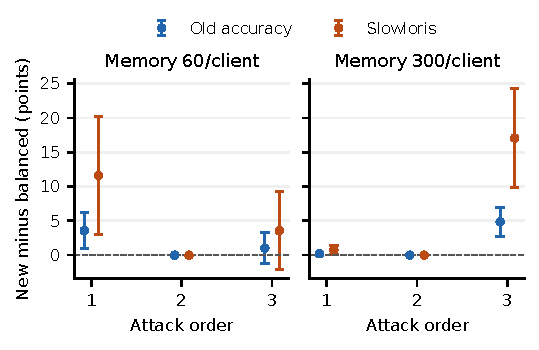
\includegraphics[width=\columnwidth]{figures/order_effects.pdf}
\caption{Federated \BR\ minus class-balanced differences by order and capacity, original split 42. Bars show paired 95\% intervals over ten seeds; zero denotes equal performance. Orders are defined in Section II.}
\label{fig:orders}
\end{figure}
Fig.~\ref{fig:orders} prevents an average improvement being interpreted as an every-order gain. At memory 60, Slowloris improves by 11.60 points $[2.99,20.21]$ in order 1, is unchanged in order 2, and improves by 3.57 $[-2.12,9.25]$ in order 3. Rare attacks are last in order 2, where both methods already achieve full Slowloris recall. Against protected, \BR\ loses Slowloris in federated orders 1 and 3 at memory 60. At memory 300 it loses old accuracy in orders 1 and 2. All capacities, environments, orders, and losses remain in the evidence.

\subsection{Benefits under federated heterogeneity}
The allocation gains persist when fitting and replay are distributed across heterogeneous clients. At memory 60, centralized \BR\ minus class-balanced differences are old accuracy $+1.67$ points $[1.12,2.22]$ and Slowloris $+5.00$ $[3.04,6.96]$. The corresponding federated gains are $+1.53$ and $+5.06$. This supports using the local policy under federation with matched total replay storage. Federated-minus-centralized differences in improvement are $-0.14$ $[-1.54,1.26]$ for old accuracy and $+0.06$ $[-4.26,4.38]$ for Slowloris; neither is significant.

\subsection{Additional splits and allocation ablation}
We repeat only class-balanced versus \BR\ at memory 60 with three additional role-split seeds, 43--45. The sampled traffic, seed-42 client allocation, original model, task orders and training settings remain fixed. For each split/order, Task-1 fitting preprocessing is refitted and frozen; both methods and environments share it. Each method selects replay settings on that split's calibration roles using the unchanged criterion, before any new evaluation. Ten training seeds and all three orders are retained.

\begin{table}[t]
\centering
\caption{Memory-60 \BR\ minus class-balanced, merged scores; percentage points [95\% paired interval]. Each row averages orders within ten paired training seeds.}
\label{tab:splits}
\footnotesize
\setlength{\tabcolsep}{3pt}
\begin{tabular}{llrr}
\toprule
Split & Setting & Old accuracy & Slowloris\\
\midrule
42 & Fed. & $+1.53$ $[0.23,2.84]$ & $+5.06$ $[1.27,8.84]$\\
42 & Central & $+1.67$ $[1.12,2.22]$ & $+5.00$ $[3.04,6.96]$\\
43 & Fed. & $+2.23$ $[0.95,3.51]$ & $+7.93$ $[4.03,11.83]$\\
43 & Central & $+1.11$ $[0.47,1.74]$ & $+3.48$ $[1.31,5.65]$\\
44 & Fed. & $+3.37$ $[2.11,4.63]$ & $+11.28$ $[7.59,14.97]$\\
44 & Central & $+1.13$ $[-0.19,2.46]$ & $+3.80$ $[-0.79,8.39]$\\
45 & Fed. & $+2.06$ $[0.40,3.72]$ & $+6.09$ $[1.30,10.88]$\\
45 & Central & $+0.82$ $[0.01,1.63]$ & $+2.61$ $[-0.01,5.22]$\\
\bottomrule
\end{tabular}
\end{table}
In the federated setting, old-accuracy differences are positive on 4/4 splits and significant on 4/4; Slowloris differences are positive on 4/4 and significant on 4/4. Worst-client differences are significantly unfavorable on 0/4. In the centralized setting, old-accuracy differences are positive on 4/4 splits and significant on 3/4; Slowloris differences are positive on 4/4 and significant on 2/4. Worst-client differences are significantly unfavorable on 0/4. Table~\ref{tab:splits} and the accompanying evidence retain every split and per-order result.

The optional rare+random policy reserves a calibrated rare share and fills the rest uniformly, with no benign minimum. On the original split, its federated differences from protected are old accuracy $-0.76$ $[-3.06,1.54]$, Slowloris $+2.05$ $[0.69,3.41]$, and worst-client $+1.47$ $[-2.19,5.12]$. Against rare+random, \BR\ changes old accuracy by $+13.45$ $[10.83,16.06]$, Slowloris by $-8.16$ $[-11.62,-4.71]$, and worst-client by $+30.41$ $[26.61,34.21]$. This comparison exposes the allocation trade-off; detailed selected quotas and all losses accompany the results.


\subsection{Focused client results}
\begin{table}[t]
\centering
\caption{Focused client results at federated memory 60. Mean percentages over seed/order runs; descriptive, without client-specific significance claims.}
\label{tab:clients}
\footnotesize
\begin{tabular}{llrr}
\toprule
Client & Method & Macro recall & Slowloris\\
\midrule
Rare-heavy & Class-balanced & 78.30 & 70.90\\
Rare-heavy & Protected & 53.99 & 81.87\\
Rare-heavy & Balanced+rare & 79.25 & 76.19\\
Benign-starved & Class-balanced & 88.58 & 75.50\\
Benign-starved & Protected & 47.56 & 85.89\\
Benign-starved & Balanced+rare & 88.55 & 79.78\\
\bottomrule
\end{tabular}
\end{table}

Table~\ref{tab:clients} reports the two profiles most directly related to the allocation motivation. At the rare-heavy client, \BR\ raises descriptive macro recall from 78.30\% with class-balanced to 79.25\%, and Slowloris from 70.90\% to 76.19\%. Protected attains 81.87\% Slowloris but only 53.99\% macro recall. The same trade-off is visible locally rather than only in pooled results.

At the benign-starved client, macro recall is effectively unchanged between balanced and \BR\ (88.58\% versus 88.55\%), while Slowloris rises from 75.50\% to 79.78\%. Protected again has higher Slowloris (85.89\%) but lower macro recall (47.56\%). These descriptive means do not imply client-specific significance. Also, the mean of per-run minima in Table~\ref{tab:main} need not equal the minimum of averaged client scores in Table~\ref{tab:clients}.

\balance
\section{Limitations}
The random role splits overlap and reuse one dataset with constructed clients; their intervals quantify training variability rather than independent capture generalization. Source filenames provide provenance groups, and flow IDs, expiration codes and timestamps are available, but no explicit session/capture column was found. The sampled traffic spans 59 scenario files, with only two benign and two Slowloris files. Whole-file assignment to three disjoint roles would leave these classes unsupported in at least one role. A file-held-out design is possible with different support/roles, but was not built in this scope.

There are only 16 benign and five fragmentation evaluation rows, so we make no false-alarm or fragmentation claims. The benign-starved profile has no benign evaluation support. Worst-client macro recall excludes unsupported labels, and non-significant intervals do not establish non-inferiority. Order-specific categorical vocabularies are fitted on the first task, so order differences mix task order and representation effects; additional splits also change fitted vocabulary. Offline shared preprocessing is not a distributed privacy protocol.

The rare+random ablation calibrates its quota while protected fixed 20\%; within-rare sampling also differs from \BR. It compares allocation policies rather than fully isolating benign-quota causality. EWC's $\lambda\in\{1,100\}$ calibration grid is limited and not a claim of optimal EWC tuning. Public FedCBDR code exists, but the inspected commit lacks directly imported modules and its README method is absent from the dispatcher; adapting the image/CUDA implementation to this tabular protocol requires reconstruction. Superiority over FedCBDR, CBRS or other untested methods is not claimed.

Intervals are unadjusted for multiple comparisons. The memory budget counts replay rows, not total process RAM. We do not evaluate deployment latency, communication cost, energy, privacy leakage, adversarial evasion, or client dropout. The memory-300 protected-over-uniform Slowloris federation interaction remains exploratory. Original capacity/order losses remain part of the evidence, and the separate larger-model exploratory tuning does not replace this fixed protocol.

\section{Conclusion}
A predeclared rare-group reservation with a balanced remainder improves old-attack retention and Slowloris recall over class-balanced replay. Both federated gains are significant on the original and each additional role split at memory 60. Matched centralized comparisons also favor the policy in direction, with significance varying across splits. The allocation ablation exposes the different retention--Slowloris trade-off of random filling. The contribution is an evaluated local replay-allocation policy for charging-network flow classification.

\begin{thebibliography}{17}
\bibitem{ocpp} Z. Garofalaki, D. Kosmanos, S. Moschoyiannis, D. Kallergis, and C. Douligeris, ``Electric vehicle charging: A survey on the security issues and challenges of the Open Charge Point Protocol (OCPP),'' arXiv:2207.01950, 2022, doi: 10.1109/COMST.2022.3184448.
\bibitem{dataset} Canadian Institute for Cybersecurity, ``CIC EV charger attack dataset 2024 (CICEVSE2024),'' University of New Brunswick, 2024. [Online]. Available: \url{https://www.unb.ca/cic/datasets/evse-dataset-2024.html}
\bibitem{diot} T. D. Nguyen \emph{et al.}, ``D\"IoT: A federated self-learning anomaly detection system for IoT,'' in \emph{Proc. IEEE ICDCS}, pp. 756--767, 2019, doi: 10.1109/ICDCS.2019.00080.
\bibitem{kitsune} Y. Mirsky, T. Doitshman, Y. Elovici, and A. Shabtai, ``Kitsune: An ensemble of autoencoders for online network intrusion detection,'' in \emph{Proc. NDSS}, 2018, doi: 10.14722/ndss.2018.23204.
\bibitem{amr} S. K. Amalapuram, S. S. Channappayya, and B. R. Tamma, ``Augmented memory replay-based continual learning approaches for network intrusion detection,'' in \emph{Advances in Neural Information Processing Systems}, vol. 36, 2023.
\bibitem{fedavg} B. McMahan, E. Moore, D. Ramage, S. Hampson, and B. A. y Arcas, ``Communication-efficient learning of deep networks from decentralized data,'' in \emph{Proc. AISTATS}, PMLR, vol. 54, pp. 1273--1282, 2017.
\bibitem{fedprox} T. Li \emph{et al.}, ``Federated optimization in heterogeneous networks,'' in \emph{Proc. MLSys}, vol. 2, 2020.
\bibitem{scaffold} S. P. Karimireddy \emph{et al.}, ``SCAFFOLD: Stochastic controlled averaging for federated learning,'' in \emph{Proc. ICML}, PMLR, vol. 119, pp. 5132--5143, 2020.
\bibitem{fedweit} J. Yoon, W. Jeong, G. Lee, E. Yang, and S. J. Hwang, ``Federated continual learning with weighted inter-client transfer,'' in \emph{Proc. ICML}, 2021, arXiv:2003.03196.
\bibitem{tiny} A. Chaudhry \emph{et al.}, ``On tiny episodic memories in continual learning,'' arXiv:1902.10486, 2019.
\bibitem{icarl} S.-A. Rebuffi, A. Kolesnikov, G. Sperl, and C. H. Lampert, ``iCaRL: Incremental classifier and representation learning,'' in \emph{Proc. CVPR}, pp. 2001--2010, 2017.
\bibitem{gem} D. Lopez-Paz and M. Ranzato, ``Gradient episodic memory for continual learning,'' in \emph{Advances in Neural Information Processing Systems}, vol. 30, 2017.
\bibitem{agem} A. Chaudhry, M. Ranzato, M. Rohrbach, and M. Elhoseiny, ``Efficient lifelong learning with A-GEM,'' in \emph{Proc. ICLR}, 2019.

\bibitem{ewc} J. Kirkpatrick \emph{et al.}, ``Overcoming catastrophic forgetting in neural networks,'' \emph{Proc. Natl. Acad. Sci. USA}, vol. 114, no. 13, pp. 3521--3526, 2017, doi: 10.1073/pnas.1611835114.
\bibitem{der} P. Buzzega, M. Boschini, A. Porrello, D. Abati, and S. Calderara, ``Dark experience for general continual learning: A strong, simple baseline,'' in \emph{Advances in Neural Information Processing Systems}, vol. 33, 2020.
\bibitem{cbrs} A. Chrysakis and M.-F. Moens, ``Online continual learning from imbalanced data,'' in \emph{Proc. ICML}, PMLR, vol. 119, pp. 1952--1961, 2020.
\bibitem{fedcbdr} Z. Qi, Y.-P. Tang, L. Meng, H. Yu, X. Li, and X. Meng, ``Class-wise balancing data replay for federated class-incremental learning,'' arXiv:2507.07712, 2025.
\end{thebibliography}
\end{document}
